% 139-12(139쪽) — 포물선 $y=x^2-1$ 과 $x$축·두 직선 $x=0$, $x=2$ 로 둘러싸인 색칠 부분(0~1 은 축 아래, 1~2 는 축 위). 스캔 화질이 낮아 TikZ 로 다시 그림.
% 원문에 있는 것만 옮긴다: 곡선 · 색칠 부분 둘 · $x=2$ 세로선 · 라벨 $-1$, O, 1, 2($x$축), $-1$($y$값), $y=x^2-1$, x, y. 원문에 없는 눈금·넓이 값은 적지 않는다.
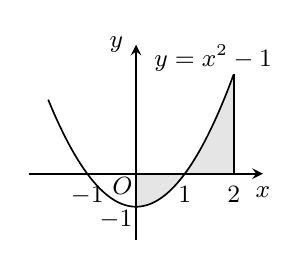
\begin{tikzpicture}[x=0.62cm, y=0.42cm, line width=0.6pt, font=\small]
  \fill[gray!20] (0,0) -- plot[domain=0:1, samples=40] (\x, {(\x)*(\x)-1}) -- (1,0) -- cycle;
  \fill[gray!20] (1,0) -- plot[domain=1:2, samples=40] (\x, {(\x)*(\x)-1}) -- (2,0) -- cycle;
  \draw[->, >=stealth, line width=0.7pt] (-2.2,0) -- (2.6,0) node[below=1pt] {$x$};
  \draw[->, >=stealth, line width=0.7pt] (0,-2.0) -- (0,3.9) node[left=1pt] {$y$};
  \draw[domain=-1.8:2.0, samples=90, smooth] plot (\x, {(\x)*(\x)-1});
  \draw (2,0) -- (2,3);
  \node[below=1pt] at (-1,0) {$-1$};
  \node[anchor=north east, inner sep=1pt] at (0,0) {$\pt{O}$};
  \node[below=1pt] at (1,0) {$1$};
  \node[below=1pt] at (2,0) {$2$};
  \node[anchor=north east, inner sep=1pt] at (0,-1) {$-1$};
  \node[anchor=west, inner sep=1pt] at (0.3,3.5) {$y=x^2-1$};
\end{tikzpicture}
